\documentclass{article}

% Language setting
% Replace `english' with e.g. `spanish' to change the document language
\usepackage[english]{babel}
% Set page size and margins
% Replace `letterpaper' with `a4paper' for UK/EU standard size
\usepackage[letterpaper,top=2cm,bottom=2cm,left=3cm,right=3cm,marginparwidth=1.75cm]{geometry}
% Useful packages
\usepackage{amsmath}
\usepackage{subcaption}
\usepackage{graphicx}
\usepackage[colorlinks=false, allcolors=blue]{hyperref}
\usepackage{booktabs}

\title{Exploring Robustness of Automated Pricing Algorithmic Collusion in Financial Markets}
\author{Ashish Rana, 1822317 \\
        ashish.rana@students.uni-mannheim.de}

\begin{document}
\maketitle
\tableofcontents % table of content
\listoftables % list of table added
\newpage

\begin{abstract}

In the modern digital economy automatically setting commodity prices for dynamically varying demands plays a huge role for maximizing the profits for an organization.
Often this helps the organizations to gain advantages over their competitors, and increase their survival rate in the market.
But, in the past it is observed that organizations often communicate and collude to maximize their profits by setting supra-competitive prices.
In the age of algorithmic pricing systems this collusion is possible without communication as well with the help of modern reinforcement learning (RL) algorithms.
And, the current antitrust laws do not explicitly prevent such possible collusion activities across different commodity markets.
With this manuscript we explore robustness of algorithmic collusion in three different RL settings, namely: i) Tabular Q-Learning, ii) Deep Q-Learning, iii) Multi-Agent Deep Q-Learning.
Also, the related code repository implementation and experimentation is present at \href{https://github.com/arana-initiatives/social-dilemma-collusion}{github.com/arana-initiatives/social-dilemma-collusion}.

\end{abstract}

\section{Introduction}

% - 1 paragraph about algorithmic collusion;
% - 1 paragraph about three studies & bigger picture;
% - 1 paragraph, more details about three studies & documentation;
With increased usage of automated pricing softwares, which holds the capacity to process data in large amounts, it is possible for firms to collude and bypass regulations.
Previously, from small scale Amazon sellers to large German retail gasoline market firms have used collusion algorithms successfully to increase price-cost margins \cite{assad2020algorithmic, kokkoris2020few}.
This problem is only going to exacerbate in the upcoming future with an ever-evolving AI landscape.
Current antitrust and competition-law targets only communication effort between firms for collusion.
And, lacks appropriate regulations to avoid collusive strategies without regulations \cite{calvano2020protecting}.
A growing literature has demonstrated the possibility of algorithmic collusion, and with this study we intend to analyze these claims in detail \cite{calvano2020artificial, klein2021autonomous}.


% - study 1 pointers
% - collusion breaks down, nash play, {coordinating -> governing} algorithm design for robust policies
% - collusion in simplistic scenario only the possibility, overfitting of collusion w/ Q-Learning, 
% - context and limits of collusion happening in that context only, forces collusion being limited to past experience of current organization, for learning simpler patterns only
% - collusion might happen beforehand w/ similar algorithms & parameterization, and market interaction acts as supplementary component

% - study 2 pointers
% - with DQN collusion is faster, reformulating state representation allows collusion in wider spaces
% - current regulations becoming useless when algorithms collude w/o communication
% - duopolies having collusion, increasing firms collusion decreases, simplifying state representations: average of past prices, defection by including min & max values of last period prices

% - study 3 pointers
% - human preferences in collusion: {up-to-date experience and RPE}; replay helps in collusion, relative performance improvement measure stabalize collusion;
% - pricing algorithm learn it is optimal to collude (Ezrachi and Stucke, 2016), Assad et al. (2020) German retail gasoline markets increasing prices, Amazon platform collusion, w/o communication collusion causing problems, 
% - temporal correlations between MDP states, firms cooperte faster with usage of past experience tuples, 
% - uniform sampling destroys collusion w/ latest buffers & random learning episodes, not all experience equally good w/ relative performance evaluation (RPE), underperformance not being considered a good scenario only force algorithms to learn from underperforming experiences, in much shorter time supera-competitive prices are reached, 
% - need to open-source or governed the code implementations, asymmetry & heterogeneity causes collusion problems,
We analyze three different studies that evaluate the same algorithmic collusion problem in different RL setups, namely: i) Tabular Q-Learning, ii) Deep Q-Learning (DQN), iii) Multi-Agent Deep Q-Learning \cite{eschenbaum2022robust, hettich2021algorithmic, han2021understanding}.
As with increasing shared novelties in colluding systems, the algorithmic collusion becomes more feasible in wider oligopolies as well.
With these three different setups, we analyze and quantify the robustness capabilities and recovery capacity in algorithmic collusion for agent firms.
For example in the first study, even though collusion is principally feasible, agents still restrict themselves to simpler strategies, like learning uniformly from their past experiences only.
Whereas in the final third study, agents supplemented with experience replay buffers give more importance to underperforming profit experiences to achieve faster supra-competitive prices with collusion.
Additionally, these studies are developed from an economic perspective, therefore experiment result interpretation is the primary focus across these studies rather than result novelties.
It further encourages interesting and practical discussion for this study to focus on real governance and regulations aspects as well instead of algorithmic novelties only.


In this manuscript, we first discuss the necessary background information regarding the used economic environment and reinforcement learning concepts.
Second, over the span of next three sections we elaborate different collusion experiment results from the above-mentioned three studies.
Third, we discuss and summarize the learnings from these studies to encourage fair and complaint competition behavior in markets with improved regulations.
Finally, we conclude our exploration study and practically quantify the learnings with social dilemma based MARL experiments. \footnote{Experimentation code available at the repository \href{https://github.com/arana-initiatives/social-dilemma-collusion}{github.com/arana-initiatives/social-dilemma-collusion}}.


\section{Background Work}


For simulating collusion scenarios, a repeated Bertrand competition model is chosen which formulates competing oligopolistic markets with homogenous goods.
This competition assumes that goods produced are identical from consumer’s perspective and the firms compete by varying prices only but not quantities.
All competitors theoretically make zero profits by selling goods at marginal cost as the goods are perfect substitutes for all competing firms.
Therefore, simulating this market scenario provides a perfect opportunity to analyze algorithmic collusion in abstract settings with minimal concept drift \cite{lu2018learning}.
In the first subsection below, we mathematically formulate the environment to specify the dynamics of repeated Bertrand competition games.
And, in the second subsection we discuss the RL problem formulation design opted by each of above mentioned studies.


% - 1 paragraph about economic environment;
% - 1 paragraph about POSG and context; other formulations & limitations
% - 1 paragraph about algorithms;

% - study 1
% - algorithms trained offline then deployed, extrapolate collusion from training w/ the market, environment parameterized by 'context', where 'context' describes change in exogenous conditions
% - POMG formulation, probability transition function & policy definition, CPOMG definition & context's capacity to capture different aspects, specifying performance of the agents
% need to elaborate repeated Bertrand setting, economic model formula with rewards, player memory in formulation {experience replay?}, collusion index and profit gain formulas, context's variations with varying marginal costs simulating information amount on demand requirements, conditional checks to avoid monopoly added
% discussion point: the variation added w/ different context, limiting and simplistic in nature only requiring change along pricing line but not across profit axis, otherwise profit payoff-pricing cost 2D axes

% - study 2
% - repeated Bertrand model competition formulation, good short description of the economic model, add description of Bertrand model competition as well
% - MDP formulation, no multi-agent setup highlighted, therefore CTCE paradigm might be opted during training, similar issue with study 1 & 3
% - discussion of average reward and updated loss function, since the reward function in Bertrand competition is having infinite horizon

% - study 3
% - temporal correlation between states, & replay buffer formulation with tuple (possibly refer introduction also)


\subsection{Economic Environment Description}


The  Bertrand competition game with two players is the baseline setup for all the experiments where players choose actions in each period t $\in$ $\{$ 0, …, T $\}$.
In time period \textit{t} for demand quantity\textit{q\textsubscript{i,t}}, the product \textit{i} follows the logit demand function specified below in equation \ref{eq:logit-demand-model}.
In vertical differentiation a firm offers products at different price points, represented in equation \ref{eq:logit-demand-model} by $\gamma$ denoting the quality parameter.
Whereas, in horizontal differentiation companies differentiate themselves by offering other products or services, represented here by $\mu$ expressing goods are perfect substitutes when $\mu$ $\rightarrow$ $\infty$.
The reward or profit at each timestep is specified by $\mathcal{R}_{i,t}$ = ($p_{i,t}$ - $c_{i}$)$q_{i,t}$.
The states \textit{S} of the system is given by price profiles (\textit{$p_{1,t},  p_{2,t}$}) like \textit{S = $A_1$ $\times$ $A_2$}, where different agent action combinations formulate the state space.
This environment uses a deterministic transition function and defines agent past memory limited to problem formulation specific horizons.


\begin{equation} \label{eq:logit-demand-model}
q_{i,t} = e^{ (\gamma_{i} - p_{i,t}) / \mu} /  \sum_{j=1}^{n} e^{(\gamma_{j} - p_{j,t}) / \mu}  + e^{\gamma_{0}/ \mu}
\end{equation} 


\begin{equation} \label{eq:collusion-index}
\mathcal{M} = \pi - \pi^{N} / \pi^{C} - \pi^{N};
\Delta_{i} = ( \pi_{i} - \pi_{i}^{N} ) / ( \pi_{i}^{C} - \pi_{i}^{N} )
\end{equation}


The collusion capabilities of algorithms are quantified by collusion index \textit{$\mathcal{M}$} and profit gain \textit{$\Delta$}, denoted by equations \ref{eq:collusion-index}.
By definition, collusion index is equal to averaged profit gains for two players involved in the baseline system.
Here, both metrics at different granularities defines: i.) average reward in relation to static Nash equilibrium, and ii.) firm profits aimed at maximizing profits.
The unique Nash equilibrium is defined over the one-shot game, where firms set their prices equal to marginal costs and make zero profit.
Therefore, using Nash equilibrium as reference for these standardized metrics is important. Because both these metrics, at \textit{$i^{th}$} firm level for \textit{$\Delta_i$} and at an average system level for \textit{$\mathcal{M}$} measures collusion tenacity.
The actions are defined in a discrete manner, where \textit{$i^{th}$} agent can choose from its action space \textit{$A_i$}.
A computationally reasonable range would be equal space prices range from the static Nash equilibrium prices \textit{$p_{i \in n}^{N}$} to monopoly prices \textit{$p_{i \in n}^{C}$} of given one-shot game.
Mathematically, the action space is defined by \textit{$A_i$} = [ min$(p_{i \in n}^{N})$ - $\xi$ , max$(p_{i \in n}^{C}$) + $\xi$ ], where $\xi$ = 0.1 * [ max($p_{i \in n}^{C}$) - min($p_{i \in n}^{N}$) ] is the markup to increase the price range by 10 \% in both directions.


\subsection{Mathematical Problem Formulation}

% write up ideas, study 1: POSG formulation, context conceptualization; my comments: advantages limited, interpretation advantages only;
% write up ideas, study 2: MDP formulation & updates in loss function; my comments: advantages limited, network convergence;
% write up ideas, study 3: MDP formulation w/ experience, multi-agent input CTCE; my comments: advantages limited, only replay experience helps;
% generral comment: still good enough, & comparable setup for analysis;
The three discussed studies formally define their collusion problem differently from theoretical perspectives while following the same centralized training and centralized execution paradigm (CTCE) paradigm \cite{papoudakis2019dealing}.
The first study formulates this problem as Partially Observable Stochastic Game (POSG).
As realistically it adheres to the belief that agents do not actually observe true underlying states in the market.
Additionally, their formulation also uses \textit{`context’ (K)} which specifies initial seeds and reward function parameters \cite{kirk2021survey}.
This helps the algorithm to jointly learn collusion in specific contexts, and it further helps in assessing collusion policy extrapolation capabilities across different contexts.
Whereas, the second study formulates the above economic environment as simple MDP, where the decision maker is the agent and everything else is considered as the environment.
This formulation is problematic since it violates Markov property theoretically, and leaves the learning system prone to overfitting with introduced non-stationarity practically.
But, to achieve faster convergence this study uses DQN with loss function formulation improvements \cite{hester2018deep}.
Since, optimal joint policy cannot be represented under this MDP formulation, we get partial order of policies.
The authors propose to formulate optimization objectives as a comparison of two policies, where the current policy is evaluated by the improvement it provides over the current true average reward estimate \cite{sutton2018reinforcement}.


The third study also formulates the problem as MDP, and practically concatenates all agent inputs in the CTCE multi-agent system during learning.
But, it exploits the temporal correlation between MDP states by using replay buffers to systematically learn from valuable past experiences \cite{zhang2017deeper}.
The second DQN based study only uses naive replay buffers, whereas the third discussed study uses ranking mechanisms to assign more value to more relevant experiences.
Practically, all three approaches use centralized executor rather than decentralized executer agents which works well in this simplistic economic environment.
The state-action pair count varies across the studies to some extent based on the price range selected in each of the studies.
But, still the qualitative findings are comparable since the underlying economic environment complexity is almost same across the baseline experiments.
And, clearly as we keep on adding additional components like deep learning networks, and experience replay buffers, we can expect the collusion to become more robust in nature.
Since, deeper and more novel RL methods can estimate the policies and value functions in a more robust manner with minimal overfitting.


\section{Robust Algorithmic Collusion}


\begin{figure}[h]
    \centering
    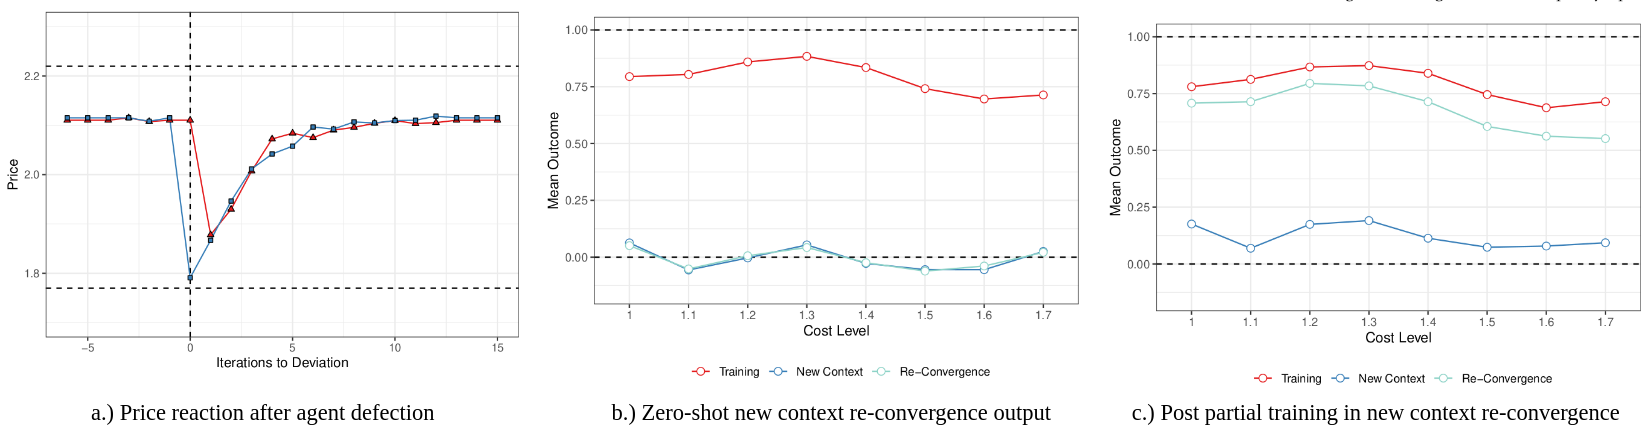
\includegraphics[width=0.99\textwidth]{study-one/collusion-reconvergence-curves.png}
    \caption{Agent strategy robustness analysis in defection scenarios and differently parameterized contexts. \textit{(Image Credit: Eschenbaum et al.)}}
    \label{fig:collusion-restore-curves}
\end{figure}


% relatively low marginal cost player willing to drive the collusion to achieve higher profits,
% but that's not the case when both players have similar marginal costs because policies might be greedy or overfitted,
% with less willingness to take profit losses qualitatively
This foundational study carries out collusion propensity experimentation in its most nascent form with baseline Q-table based learning.
But, uniquely enough this study defines the \textit{`context’} concept, which varies in marginal cost values for tuning the experiments to different marginal cost parameters.
Also, across all the training contexts with varying cost, a high collusion index between 0.70 and 0.87 is observed with highly symmetric profit gains for agents.
For convergence approximately million plus timesteps are taken across all contexts on an average.
This makes the collusion amongst agents highly unfeasible in realistic market setups.
Experimentally it is further observed that players with high cost level lose when best response Nash play happens, and opt to reduce their prices.
Vice-versa, players in low cost contexts show tendency to achieve above-Nash profits against Nash plays, which restores collusion, as highlighted in Figure \ref{fig:collusion-restore-curves}.a.
In the Figure \ref{fig:collusion-restore-curves}.a, agent is forced for the price defection, and the second agent punishes the defecting agent with its price drop before returning to stable pre-deviation collusion prices.
Further, to measure the collusion generalization capabilities this study trains the model in different context, and tests the collusion propensity in another context having different cost parameters as shown in Figure \ref{fig:collusion-restore-curves}.b and Figure \ref{fig:collusion-restore-curves}.c.
From these Figures, we observe that if we directly evaluate the collusion models in different contexts the collusion breaks.
But if we allow continued training or fine-tuning to some extent, the collusion plot again highlights reconverges back to near ideal collusion levels as earlier.


\begin{figure}[h]
    \centering
    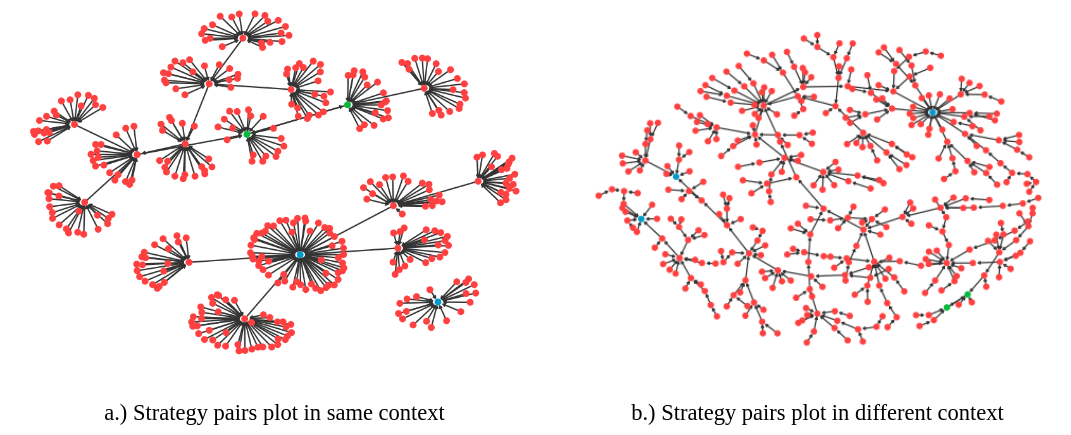
\includegraphics[width=0.75\textwidth]{study-one/transitive-strategy-pairs.png}
    \caption{Agent strategy transitive closure plots for strategy evaluation in similar and different contexts. Here, the blue nodes highlight stable end-nodes with fixed action strategies, and green nodes highlight unstable end-nodes with cycles of varying action strategies. \textit{(Image Credit: Eschenbaum et al.)}}
    \label{fig:transitive-strategy-pairs}
\end{figure}


\begin{figure}[h]
    \centering
    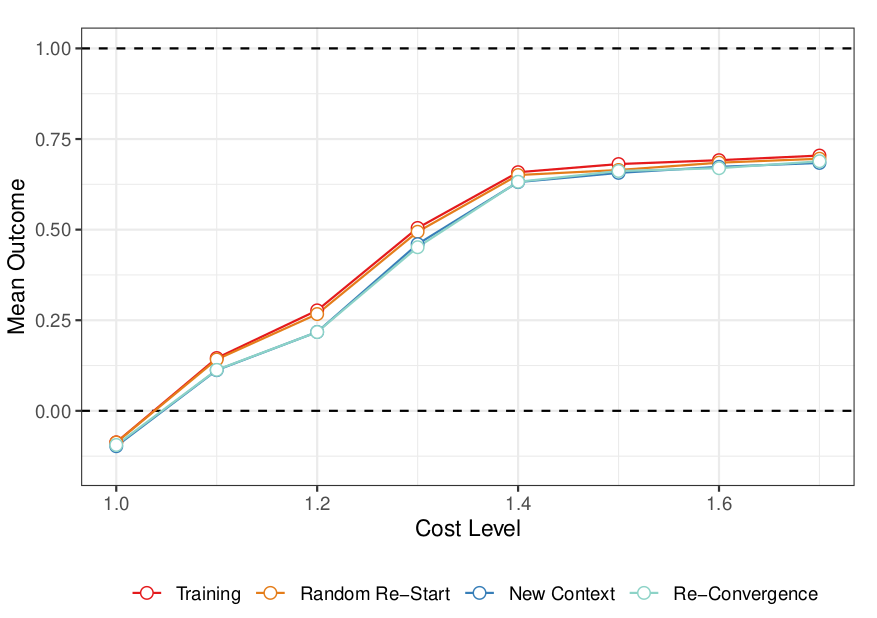
\includegraphics[width=0.4\textwidth]{study-one/restricted-observation-space.png}
    \caption{Collusion convergence and re-convergence plots in restricted observation space during training and evaluation in new context. \textit{(Image Credit: Eschenbaum et al.)}}
    \label{fig:restricted-observation-space}
\end{figure}


From a game theory interpretation perspective this study also plots transitive closure of the strategy pairs. 
As after the convergence, theoretically an agent plays pure strategy having a single action corresponding to each observation state which can be discretely represented and plotted.
In Figure \ref{fig:transitive-strategy-pairs}, each node represents an observation state, and the edge represents the transition that occurs from the strategy pair for the agents in the joint policy.
We can see different variations in these plots for the same parameterization context if the initial seeds are different but all of them are robust to defections.
Further, the strategy pairs are also evaluated in different testing contexts, where we observe overfitted complex transitive closure plots as highlighted in Figure \ref{fig:transitive-strategy-pairs}.b.
With these different transitive closure plots observations, it is concluded that agents are not learning the complete convergence strategies/policies but rather only learn their approximations.
Therefore, the authors attempt to reduce the policy strategy space where agents only observe their own past action price.
Figure \ref{fig:restricted-observation-space}, demonstrates average profit gains for different cost prices with this reduced state formulation.
We observe that with this state simplification, agent’s collusion propensity increases across all the evaluation contexts when marginal cost prices are high.
This highlights the increased tendency to gain more rewards when high profit gains are involved otherwise the agent prefers the equilibrium state.


\section{Algorithmic Collusion: Insights from Deep Learning}


\begin{figure}[h]
    \centering
    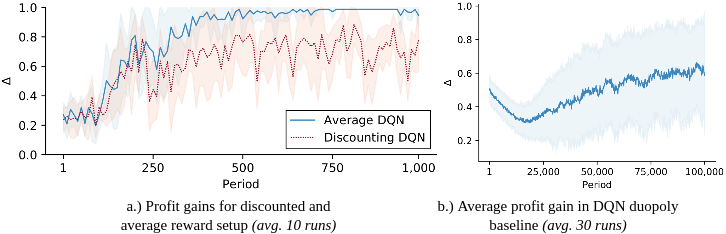
\includegraphics[width=0.7\textwidth]{study-two/learning-curves-merged.png}
    \caption{Average profit gain curves for measuring collusion propensity in baseline duopoly markets. \textit{(Image Credit: Hettich et al.)}}
    \label{fig:learning-curves-merged}
\end{figure}


This study conducts similar experiments as the first study to measure different aspects of collusion propensity and robustness.
In the previous study, the collusion converged approximately after a few million timestep iterations across different contexts.
On an average with DQN model usage in the current study it converges around at 850,000 timesteps.
Clearly, with usage of DQN models the convergence happens relatively faster, as more parameters are available for better approximation of policies.
Second from Figure \ref{fig:learning-curves-merged}.a, we also observe that loss function reformulation by using average rewards for averaged DQN learning provides more stabilization in the learning process.
Whereas, the discounting DQN keeps on looking for a better partial order policy set and keeps on overfitting.
This further destabilizes the learning process which results in oscillating behavior around several lower optima values.
The DQN implementation consists of exploration factor $\varepsilon$, which when decreases the agent actions become less explorative, which in turn stabilizes convergence curves.
The Figure \ref{fig:learning-curves-merged}.b, shows that as part of initial exploration strategy the agents often opt for price undercuts leading to almost static Nash equilibrium.
And, finally with decreasing $\varepsilon$ the agents turn towards collusion convergence in the given duopoly baseline setting.


\begin{figure}[h]
    \centering
    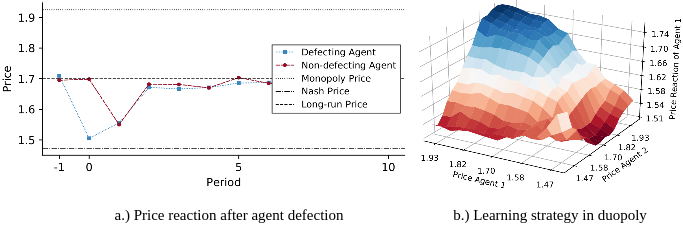
\includegraphics[width=0.7\textwidth]{study-two/defection-strategy.png}
    \caption{Agent strategy analysis and interpretation summary. \textit{(Image Credit: Hettich et al.)}}
    \label{fig:defection-strategy}
\end{figure}


Supra-competitive prices highlight that either a firm's competitive advantage or anti-competitive market behavior has driven market goods to non-sustainable prices.
In this problem’s context, it means supra-competitive prices are set when either some agents fail to compete effectively or the agents learn effective reward-punishment policies for collusion.
From Figure \ref{fig:defection-strategy}.a, we observe that with added manual Nash equilibrium price defection, the second agent also lowers its price to undo the first defecting agent’s advantage.
The first defecting agent lower its future prices expecting this punishment, and further both agents iteratively start increasing their prices towards a supra-competitive price setting.
The action space size is 15 for each agent in this study, and the average agent strategy for the whole state-space \textit{(15 $\times$ 15 )} is computed in Figure \ref{fig:defection-strategy}.b.
The general symmetry in the surface highlights that DQN agents react similarly to previous prices irrespective of which agent played which price.
We can utilize Figure \ref{fig:defection-strategy}.b to interpret Figure \ref{fig:learning-curves-merged}.b experiment, the first player also defects \textit{(low z-axis price value)} after it has detected punishment state of the second agent \textit{(low x-axis price value)} when collusion with agent one \textit{(high y-axis price value)} already existed.
Additionally, the prices also increase when both agents near the Nash price, this further assists the agents to return for higher prices after the action-reaction punishment cycle.


\begin{figure}[h]
    \centering
    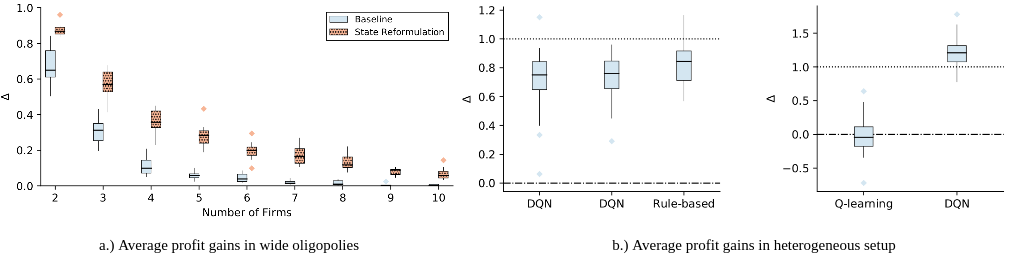
\includegraphics[width=0.95\textwidth]{study-two/additional-experiments.png}
    \caption{MARL mobile robot framework pipeline for warehouse management. \textit{(Image Credit: Hettich et al.)}}
    \label{fig:additional-experiments}
\end{figure}


Previously, we have seen collusion is strongly affected by the number of competitors, and the difference in \textit{`context’} i.e. heterogeneity in agent parameterization.
With Figure \ref{fig:additional-experiments}.a, we observe that here also with DQN, collusion is harder to sustain as the number of agents increases.
But, the collusion capacity is still larger here in comparison to Q-table learning discussed in the first study.
More importantly with state reformulation simplification, which considers only overall price and whether agent has defected results in collusion propensity improvement as highlighted in \ref{fig:additional-experiments}.a.
Further Figure \ref{fig:additional-experiments}.b elaborates on the experiment analyzing the impact of heterogeneous agents in automated collusion.
First from the right subplot in FIgure \ref{fig:additional-experiments}.b, we observe that simple baseline Q-table learning is unable to compete with a relatively novel DQN approach.
Additionally, in the left subplot with another added simple price mimicking rule-based agent, the collusion profit gains are unaffected and the collusion index matches duopoly scenarios even with added extra agent.
Like the first study, this experiment highlights the need for homogeneity in agents for symmetric collusion to exist, or otherwise some agents might end up becoming relatively incompetent.


\section{Algorithmic Collusion with Experience Replay}


% For MARLS temporal correlation helps in maintaining stationarity, importance of replays
% C-Random & D-Random breaks correlations, and DQN does not learn order, non-stationarity is weak
% different analyzed algorithm types in tabular form, destable collusion and recovering collusion

% one paragraph each for destabalizing collusion and hetergeneous players
In past studies it has been observed that strong temporal correlation from the past helps in maintaining environment stationarity, whereas random experience replay leads to non-stationarity \cite{leibo2017multi, foerster2017stabilising}.
This study utilizes this insight to deploy a replay buffer that assigns more value to near past experiences that yield higher average profit gains.
Like the above discussed studies, this study also compares different aspects like collusion propensity, robustness, and heterogeneity in their experimentation.
The Table \ref{table_algorithm_description} gives a functional description of the handy algorithm notations used in this study during the different experiments.


From Figure \ref{fig:rank-replay-experiments}.a, we observe that Q-Table based algorithms after convergence do select higher prices in general.
The percentage axis highlights the fraction of simulation runs which converge at a given average price point for C-Online, C-Random, and C-Rank algorithms.
Similar to findings in the first study, the C-Online equivalent baseline does set high prices for a relatively large number of simulation runs.
But, C-Random with random updates and C-Rank with profit gain based updates are able to explore higher price convergence prices.
With C-Rank algorithm’s capability to find highest prices for relatively larger numbers of simulation runs, its defection behavior in deep learning setup is also analyzed.
From Figure \ref{fig:rank-replay-experiments}.b, we observe that D-Rank quickly converges to supra-competitive prices by exploiting the knowledge from experiences where the agent fails to gain profits.
Clearly, the fraction of prices below 1.79 drops immediately under 1000 episodes and both players settle for very high prices to get large profit gains.
Additionally, the greedy policy matrix values highlighted in the second study are all at high constant value.
Which means that after defection, both agents immediately restore their pre-deviation price without incurring any punishment.
The non-defecting agent optimistically keeps the commodity price values high to tempt the agent to immediately switch to pre-deviation collusion price.


\begin{table*}[t]
\centering
\caption{Functional description of the different algorithms used for collusion experimentation tasks.}
     \label{table_algorithm_description}
    \begin{center}
        \begin{tabular}{ll}
        \toprule
            Algorithm Name & Functional Description \\
        \midrule 
             C-Random & Randomly updates the previous experience tuple cell \\
             C-Online & Updates the current observed state cell \\
             C-Rank & Updates the state cell when profit does not exceed competitor \\
             D-Random & DQN updating all cells, doesn't learn order of samples  \\
             D-Online & DQN using recent most data from replay buffer \\
             D-Rank & DQN using best reward gain experiences from replay buffer for profit gains \\
        \bottomrule
        \\
       \end{tabular}
     \end{center}
\end{table*}


\begin{figure}[h]
    \centering
    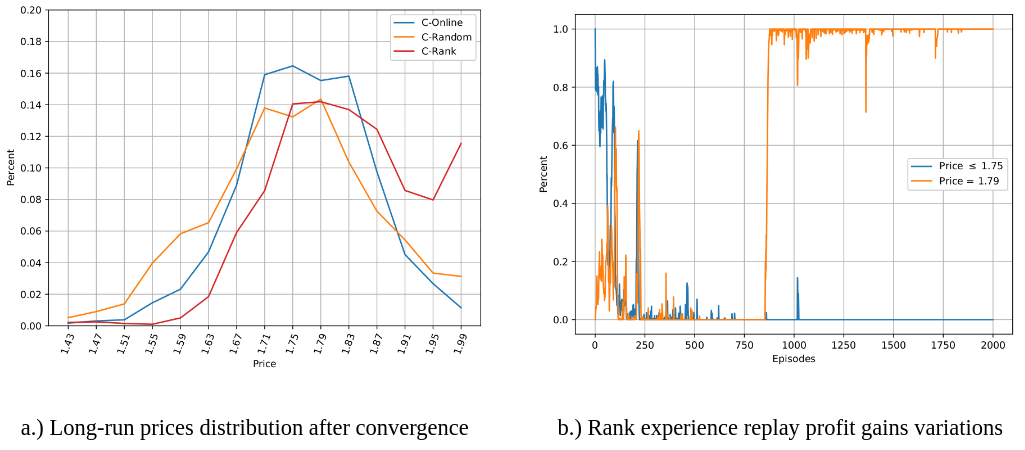
\includegraphics[width=0.65\textwidth]{study-three/rank-replay-experience-experiments.png}
    \caption{Rank experience replay price and profit gain variations summary. \textit{(Image Credit: Han et al.)}}
    \label{fig:rank-replay-experiments}
\end{figure}


For heterogeneous agent comparison parameterized by different algorithms, it is observed that more novel algorithms are able to increase their corresponding average prices relatively easily.
Specifically, the deep variants of the algorithms outperform their Q-table counterpart in terms of their individual profit gains.
This already confirms the correlation trend between algorithm novelty and collusion propensity that is observed in the above discussed studies.
Additionally, experience ranking algorithms dominate random and online agents to set supra-competitive prices.
This form of collusion where one entity clearly drives profits with its algorithmic advantage causes legal ambiguity in a real world setting.
Even though collusion persists practically, legally we can quantitatively calculate: i.) which firm to what extent is responsible for colluding, ii.) and what exactly should be the methodology to specifically penalize a firm.


\begin{table*}[t]
\centering
\caption{Cost asymmetry where marginal cost of efficient Player 2 reduces to 0.5.}
     \label{table_firm_asymmetry}
    \begin{center}
        \begin{tabular}{ccccc}
        \toprule
            Strategy & C-Online & C-Rank & D-Random & D-Rank \\
        \midrule 
             Player 1 & 1.95 & 1.55 & 1.40 & 1.65 \\
             Player 2 & 1.70 & 1.60 & 1.25 & 1.75 \\
        \bottomrule
        \\
       \end{tabular}
     \end{center}
\end{table*}


% important additional experiments: robustness discussion
Similar to previous studies as observed from Table \ref{table_firm_asymmetry}, the asymmetry in firms reduces the average profit gains when compared with symmetric firms experiments.
The inefficiency of the D-Random algorithm still persists as it maintains prices close to Bertrand equilibrium.
Whereas, C-Online algorithms like shown in previous discussed studies suffer from collusion profit gain reduction to a limited extent.
Whereas, for C-Rand and D-Rank algorithms the more efficient firm prioritizes its profits rather than increasing the average profit gains.


\begin{table*}[t]
\centering
\caption{Convergence result summary under different initializations with larger action space having higher upper bound than monopoly prices.}
     \label{table_different_initializations}
    \begin{center}
        \begin{tabular}{cccccc}
        \toprule
            Initialization & Baseline & Q = 0 & Random & Q = 19 & Topmost \\
        \midrule 
             D-Random & Bertrand & Bertrand & Bertrand & Bertrand & Bertrand \\
             D-Rank & High & High & High & High & High \\
             C-Rank & High & Upper Bound & Upper Bound & High & Volatile \\
        \bottomrule
        \\
       \end{tabular}
     \end{center}
\end{table*}


Different initialization yields different optima in deep learning problems, therefore it is important to analyze which initialization is optimal or truly non-informative \cite{sutskever2013importance}.
The Table \ref{table_different_initializations} highlights different initializations for Q-values, namely: i) baseline He initialization values, ii) zero Q-values, iii) uniform random values, iv) large constant values, v) zero Q-values except for highest price entries.
\cite{he2015delving}.
The deep network based algorithms are robust to all initializations, the D-Random still fails to learn collusion whereas the D-Rank always learns to collude.
The C-Rank shows high sensitivity to initialization values, like it learns to collude for baseline initializations similar to above two discussed studies.
For the C-Rank algorithm, \textit{`Upper Bound’} convergence represents above monopoly prices, and \textit{`Volatile’} convergence expresses instability in learning prices.
The C-Rank shows high dependency on the convergence properties based on priori information.
Essentially meaning that the C-Rank algorithm owing to its high temporal correlation issue is vulnerable to settling for local minimas.


\section{Discussion and Conclusion}


% in our case study, we highlight the similar experiments across different architectures
% collusion without explicit instruction issue, algorithms can learn good strategies
% address issue of offline training market being non-identical than the original one
% overfits, vanishes in new context & needs more information, restricting strategy space helps
With these studies by using a standard benchmark environment and similar experiments, we can clearly observe the feasibility of collusion in real market systems.
\footnote{Bibliography papers available at the repository \href{https://github.com/arana-initiatives/ai-portfolio-bibliography}{github.com/arana-initiatives/ai-portfolio-bibliography}.}
Similar experiments testing collusion propensity, robustness, and heterogeneous agent effect across three RL algorithm implementations, helps us in systematically analyzing the collusion systems.
First, we observe that with increased novelty the collusion convergence drops drastically from 850k to 2K timesteps.
Second, with deep learning based systems the collusion can exist in wider oligopolies as well, and the propensity increases with representation simplification.
Further, the experiments highlight that the market agents are capable of learning different strategies for collusion re-convergence.
For example, first demonstrating reward-punishment behavior after agent price defection, and second showcasing optimistic high price behavior when ranked replay information is available.
Finally, for heterogeneous agents we observe that more novel agents drive the collusion to gain more profit.
But, the less novel agents are also forced to place prices above the equilibrium price.
These experiments highlight that collusion with simple deep learning based RL algorithms, like DQN can help achieve collusion in minimalist formal economic environments.
The practical application translation of such insights still needs to be further analyzed considering different realistic aspects.
For example, \textit{`sim-to-real’} or \textit{`concept drift’} challenges might arise as the economic environment does not operate in isolation, but rather shows dependencies to other markets as well \cite{lu2018learning, zhao2020sim}.


% faster collusion, even faster possibe reaslistically {800K, 20K}
% human agent involved, still collusion is possible
% hetergeniety important factor, decides extent of collusion
% continous spectrum of prices, temporary character of prices in real-world important
% quick adaptation with meta-learning (wang2018prefrontal), & quick restart in fast changing markets
Realistically, there are several limitations for the discussed studies, and the limited insights that these studies provide for the algorithmic collusion task.
First, the economic benchmark environment models only Bertrand competition which just varies the prices, but realistically firms can also vary their quantities like in Stackelberg competition \cite{julien2011note}.
Additionally, the prices selected are from discrete and limited intervals which simplifies the problem significantly which might not be the case in real life scenarios.
Second, the actions are executed from a centralized controller, and agents observe the whole system in a given interval.
Practically, the agent firms would not have access to the exact reward scheme defined by other competitive firms for tuning their pricing algorithm.
This simple setting might be problematic as economic markets being related to other markets might not observe the exact underlying state, and the agents in the multi-agent systems will have their own executor unit.
The above listed studies do not discuss the economic systems in such extensive detail algorithmically but rather focus on the interpretability of selected policies.
The stability and interpretation insights of these policies, although useful, might not generalize over pricing systems built with deeper and more novel blackbox RL algorithms.
The insightful developments from deployment of these advanced systems are not measured in the existing algorithmic collusion literature.
Further, the algorithms used in the studies are also not the most novel algorithms being used by any industry or academia standard.
Therefore, it might be possible that more novel algorithms can assist agents in even faster
collusion, and help firms learn even better agent defection reaction strategies.
This would be highly problematic for regulatory authorities, as even after breaking the collusion, the firms would be capable of formulating a new near immediate automated collusion strategy.
Finally, only the first study extensively explores the impact on collusion propensity by evaluating already trained agents on different contexts i.e. baseline zero-shot learning performance, and few-shot learning performance for re-convergence.
Hence, more experiments studying zero-shot and few-shot collusion performance would give more insights into the robustness of deep learning based RL models for collusion re-convergence.


% D-Random agents dilemma, baseline that in hetergenous setting does not collude but can gain profits, how much is its associated liability
% three studies conclude differently, based on the deployed novelty in solution
Practically, it is still incredible that agents are able to collude at such a fast pace without any explicit communication and coordination protocol.
Further, to supplement the algorithm performance for ever changing markets, meta-learning can also be explored as an additional information supplementation module for collusion \cite{wang2018prefrontal}.
Since, the product and its associated price life cycles are small for a huge range of commodities.
Hence, it would be important to study and test automated collusion algorithms that allow immediate collusion restarts and direct transference across different products and markets.
Human colluders and price setters are also involved in the pricing markets, and experiments involving heterogeneous human agents would help to quantify the capabilities of the collusion algorithms more accurately.
From a regulation perspective it is very hard to detect such collusions without the knowledge of algorithms, architectures and parameterizations of the models involved.
Therefore, the regulatory bodies must enforce regulations on firms to disclose their algorithms to supervising bodies to encourage fair competition \cite{glauner2022assessment}.
Second, the legal framework for determining liability of firms involved in such malpractices should also be well-defined with minimal ambiguity.
Since, in heterogeneous agent environments more novel algorithms drive the collusion but other firms also charge higher prices.
Therefore, the extent of firms involved voluntarily or involuntarily should be determined, and based on antitrust behavior and profit gains intent the liability should be determined.
With huge amounts of data the ideal collusive strategies, economically can drive the prices to near monopolistic prices with automated pricing algorithms.
Therefore, these anti-competent practices should also be regulated under the monopoly antitrust laws as well \cite{ma2022regulating}.


With increasing novelty in algorithms across studies, we observed that the firms can collude at a much faster and practically reasonable rate.
The current literature certainly analyzes the situation in a simplistic setting with baseline RL models.
But, current RL literature and algorithms are capable of handling far more realistic and complex scenarios at a much faster rate.
For automated collusion with involvement of heterogeneous parties, determining the extent of responsibility and liability for increased collusion propensity is also ambiguous.
Therefore, it is safe to assume that near future deployment of these algorithms in different commodity markets will be a major problem.
In conclusion, these automated algorithms do pose serious threats in future to generate collusive market strategies, and promote antitrust behavior amongst the involved firms.
Hence, involvement of supervising authorities for regulations, more transparency around usage of these algorithms, and design of democratized platforms that discourage such collusion efforts is very important \cite{noothigattu2019teaching}.


\bibliographystyle{acm}
\bibliography{main}

\end{document}


% Important Links: 

% 1. Bertrand Competition: https://inomics.com/terms/bertrand-competition-1504578
% 2. Multi-agent Inaccuracies: https://agents.inf.ed.ac.uk/blog/multiagent-rl-inaccuracies/
